\RequirePackage{mmap}  % make PDF copy and paste-able
\documentclass[twocolumn]{article}
\usepackage{amsmath, amsthm, amssymb}
\usepackage{mathrsfs}
\usepackage[utf8]{inputenc}
\usepackage[T1]{fontenc}
% \usepackage{lmodern} % from http://tex.stackexchange.com/a/115089/121234
\usepackage[margin=0.3in]{geometry}


\setlength{\parskip}{0ex}
\usepackage{ragged2e}
  \setlength{\RaggedRightParindent}{1em}

\usepackage{url}
\usepackage{listings}
\lstset{%
  basicstyle=\scriptsize\ttfamily,  % the size of the fonts 
  columns=fixed,          % anything else is horrifying
  showspaces=false,       % show spaces using underscores?
  showstringspaces=false, % underline spaces within strings?
  showtabs=false,         % show tabs within strings?
  xleftmargin=1.5em,      % left margin space
}
\lstdefinestyle{inline}{basicstyle=\ttfamily}

\usepackage[dvipsnames]{xcolor}
  \definecolor{headcolor}{HTML}{004225} % British racing green {E34234}  % vermillion
  \definecolor{lightblue}{HTML}{5F9EA0} % Light blue color
  \definecolor{rosered}{HTML}{FF007F} % Rose red color
  \definecolor{subheadcolor}{HTML}{09B000} % Light green color
\usepackage{titlesec}
% \titleformat{ command }[ shape ]{ format }{ label }{ sep }{ before-code }[ after-code ]
% \titlespacing*{ command }{ left }{ before-sep }{ after-sep }[ right-sep ]
\titleformat{\section}[runin]{\color{headcolor}\bf}{}{0em}{}
  \titlespacing*{\section}{0em}{0.65ex}{0.67em}
\titleformat{\subsection}[runin]{\color{subheadcolor}\bf}{}{0em}{}
  \titlespacing*{\subsection}{0em}{0.60ex}{0.62em}

\usepackage{pdfpages}
\usepackage{graphicx} % For including images (PDFs, etc.)
\usepackage{wrapfig}  % For wrapping text around figures

% TODO
\newcommand{\method}[1]{\textbf{\textcolor{lightblue}{#1}}}
\newcommand{\sectionspace}{\vspace*{1em}}
\newcommand{\sectionLargeSpace}{\vspace*{10em}}
\newcommand{\properties}[1]{\textbf{\textcolor{rosered}{#1}}}


\pagestyle{empty}
\begin{document}\thispagestyle{empty}
\RaggedRight
\begin{center}
  {\large\color{headcolor}\textbf{SVCDE by Yiding 2024.11.17}}  \\
\end{center}

\section{Partial  Derivatives}
:\\
1. \textbf{Level curves} are the curves with equations $f(x,y) = k$ where $k$ is a constant\\
2. \method{METHOD - Limit of $f(x,y)$}: The limit $\lim_{(x, y) \to (a, b)} f(x, y) = L$ exist when all pass to (a, b) give the same result.  some useful path: $x = 0$, $ y = 0$, $y = x$, $y = x^2$\\
3. \textbf{Clairaut's Theorem:} Suppose $f$ is defined on a disk $D$ that contains the point $(a, b)$. If the functions $f_{xy}$ and $f_{yx}$ are both continuous on $D$, then
$f_{xy}(a, b) = f_{yx}(a, b)$\\
4. \method{METHOD - Tangent Plane}: $z - z_0 = f_x(x_0, y_0)(x - x_0) + f_y(x_0, y_0)(y - y_0).$\\
5. \method{\textbf{Chain Rule 2}}: Suppose that \( z = f(x, y) \) is a differentiable function of \( x \) and \( y \), where \( x = g(s, t) \) and \( y = h(s, t) \) are differentiable functions of \( s \) and \( t \). Then$\frac{\partial z}{\partial s} = \frac{\partial f}{\partial x} \frac{\partial x}{\partial s} + \frac{\partial f}{\partial y} \frac{\partial y}{\partial s}$ and $\frac{\partial z}{\partial t} = \frac{\partial f}{\partial x} \frac{\partial x}{\partial t} + \frac{\partial f}{\partial y} \frac{\partial y}{\partial t}$\\
6.\method{Chain Rule 1}: $\frac{dz}{dt} = \frac{\partial f}{\partial x} \frac{dx}{dt} + \frac{\partial f}{\partial y} \frac{dy}{dt}$\\
7. \method{\textbf{The directional derivative}} of \( f \) at \( (x_0, y_0) \) in the direction of a unit vector \( \mathbf{u} = (a, b) \) is $D_{\mathbf{u}} f(x_0, y_0) = \nabla f(x_0, y_0) \cdot \mathbf{u} =  f_x(x_0, y_0) a + f_y(x_0, y_0) b$ if this limit exists.\\
8. \textbf{Gradient vector $\nabla f(x, y)  = f_x \mathbf{i} + f_y \mathbf{j}$}\\
9. \method{METHOD - Second derivative test to find the property of a critical point (\properties{$\mathbb{R}_2$})}: \\
$
D_{2,2} = \begin{vmatrix}
	f_{xx} & f_{yx} \\
	f_{xy} & f_{yy}
\end{vmatrix}
= f_{xx}f_{yy} - (f_{xy})^2
$\\
if at point $(a,b)$, $f_{x}(a,b) = 0$ and $f_{y}(a,b) = 0$ then $(a, b)$ is a critical point that:\\
- If $D_{2,2} > 0$ and $f_{xx}(a, b) > 0$, then $f(a, b)$ is a local minimum.\\
- If $D_{2,2} > 0$ and $f_{xx}(a, b) < 0$, then $f(a, b)$ is a local maximum.\\
- If $D_{2,2} < 0$ then $f(a, b)$ is not a local maximum or minimum.\\
(Saddle Point)\\

10. \method{Critical Point(\properties{$\mathbb{R}_{3}$})}\\

-If \( D_{1,1} > 0 \), \( D_{2,2} > 0 \), \( D_{3,3} > 0 \), then \( f(a, b, c) \) is a local minimum.\\
-If \( D_{1,1} < 0 \), \( D_{2,2} > 0 \), \( D_{3,3} < 0 \), then \( f(a, b, c) \) is a local maximum.\\
-If \( D_{3,3} \neq 0 \) and \( (a, b, c) \) is neither a local minimum nor a local maximum, then \( (a, b, c) \) is a saddle point.\\
-If \( D_{3,3} = 0 \), then the test is inconclusive; \( f(a, b, c) \) could be a local maximum or minimum, or \( (a, b, c) \) could be a saddle point.\\





11. \method{METHOD : Find ABSOLUTE maximum or minimum}:\\
- find all the value of critical point\\
- find extreme value on boundary\\
- compare them\\

\sectionspace
\sectionspace

12.\method{METHOD: Lagrange multipliers}:\\
$\nabla f(x,y,z) = \lambda \nabla g(x,y,z))$\\
$g(x, y, z) = k$ (constraint)

\sectionspace

\section{Multiple integral}
:\\
1. \method{\textbf{Polar Coordinates}}:\\ $\iint\limits_R f(x, y) \, dA = \int_\alpha^\beta \int_a^b f(r \cos \theta, r \sin \theta) \, r \, dr \, d\theta$\\
2. \method{\textbf{Cylinder Coordinates}}:\\ $\iiint\limits_E f(x, y, z) \, dV = \int_\alpha^\beta \int_{h_1(\theta)}^{h_2(\theta)} \int_{u_1(r \cos \theta, r \sin \theta)}^{u_2(r \cos \theta, r \sin \theta)} f(r \cos \theta, r \sin \theta, z) \, r \, dz \, dr \, d\theta$\\
3. \method{\textbf{Spherical Coordinates}}:\\ $\iiint\limits_E f(x, y, z) \, dV = \int_c^d \int_\alpha^\beta \int_a^b f(\rho \sin \phi \cos \theta, \rho \sin \phi \sin \theta, \rho \cos \phi) 
\, \rho^2 \sin \phi \, d\rho \, d\theta \, d\phi$
4. \textbf{Jacobian}:\\
$
\frac{\partial(x, y)}{\partial(u, v)} = 
\begin{vmatrix}
	\frac{\partial x}{\partial u} & \frac{\partial x}{\partial v} \\[8pt]
	\frac{\partial y}{\partial u} & \frac{\partial y}{\partial v}
\end{vmatrix}
= \frac{\partial x}{\partial u} \frac{\partial y}{\partial v} - \frac{\partial x}{\partial v} \frac{\partial y}{\partial u}
$\\
5. \method{\textbf{Change of variables}}:\\
$\iint\limits_R f(x, y) \, dA = \iint\limits_S f(x(u, v), y(u, v)) 
\left| \frac{\partial(x, y)}{\partial(u, v)} \right| \, du \, dv$

\section{Vector Calculus}

\subsection{Line Integral}
:\\
1. \method{\textbf{Line Integral with respect to Arc length}}:\\
 $\int_C f(x, y) \, ds = \int_a^b f(x(t), y(t)) 
\sqrt{\left( \frac{dx}{dt} \right)^2 + \left( \frac{dy}{dt} \right)^2} \, dt$\\
2. \method{\textbf{Line Integral with respect to $x$ or $y$}}:\\
$\int_C f(x, y) \, dx = \int_a^b f(x(t), y(t)) \frac{dx}{dt} \, dt$\\
$\int_C f(x, y) \, dy = \int_a^b f(x(t), y(t)) \frac{dy}{dt} \, dt$\\
3. \method{\textbf{Line segment start at $\mathbf{r}_{0}$ and end at $\mathbf{r}_{1}$}}:\\
$\mathbf{r}(t) = (1 - t)\mathbf{r}_{0} + t\mathbf{r}_{1}, $\\
4. \method{\textbf{Line segment of Vector Field}}:\\
$\int_C \mathbf{F} \cdot d\mathbf{r} = \int_a^b \mathbf{F}(\mathbf{r}(t)) \cdot \mathbf{r}'(t) \, dt$\\
5. \method{\textbf{Green's Theorem}}:\\
$\oint_C \mathbf{F} \cdot d\mathbf{r} = \iint\limits_D \left( \frac{\partial Q}{\partial x} - \frac{\partial P}{\partial y} \right) \, dA$

\subsection{surface integral}
:\\
1. \method{\textbf{Surface Integralf of $f$ over the surface $S$}}:\\
$\iint\limits_S f(x, y, z) \, dS = \iint\limits_D f(\mathbf{r}(u, v)) 
\left| \mathbf{r}_u \times \mathbf{r}_v \right| \, dA
$\\
2. \method{\textbf{Surface Integral of Vector Field}}:\\
$\iint\limits_S \mathbf{F} \cdot d\mathbf{S} = \iint\limits_D \mathbf{F}(\mathbf{r}(u, v)) \cdot (\mathbf{r}_u \times \mathbf{r}_v) \, dA$\\
$\iint\limits_S \mathbf{F} \cdot d\mathbf{S} = \iint\limits_D \left( -P \frac{\partial g}{\partial x} - Q \frac{\partial g}{\partial y} + R \right) \, dA$, $g(x,y) = z$\\
3. \method{\textbf{Stoke's Theorem}}:\\
$\oint_C \mathbf{F} \cdot d\mathbf{r} = \iint\limits_S \left( \nabla \times \mathbf{F} \right) \cdot d\mathbf{S}$\\
4. \method{\textbf{Divergence Theorem}}:\\
$\iiint\limits_E \nabla \cdot \mathbf{F} \, dV = \iint\limits_S \mathbf{F} \cdot d\mathbf{S} = \iint\limits_S \mathbf{F} \cdot \mathbf{n} \, dS $\\
Where $\mathbf{n} = \frac{\mathbf{r}_u \times \mathbf{r}_v}{|\mathbf{r}_u \times \mathbf{r}_v|}$

\subsection{Parametric Surface}
:\\
1. \method{\textbf{Sphere($a$ as a constant)}}:\\
$x = a \sin \phi \cos \theta, y = a \sin \phi \sin \theta, z = a \cos \phi$\\
$\mathbf{r}_\phi \times \mathbf{r}_\theta = a^2 \sin^2 \phi \cos \theta \, \mathbf{i} + a^2 \sin^2 \phi \sin \theta \, \mathbf{j} + a^2 \sin \phi \cos \phi \, \mathbf{k}$\\
$|\mathbf{r}_\phi \times \mathbf{r}_\theta| = a^2 \sin \phi$\\

2. \method{surface area}:\\
$\iint\limits_S dS = \iint\limits_D \left| \mathbf{r}_x \times \mathbf{r}_y\right| \, dA$; 
$\iint\limits_S dS = \iint\limits_D \sqrt{1 + (\frac{\partial{z}}{\partial{x}})^2 + (\frac{\partial{z}}{\partial{y}})^2} \, dA$, when $z = g(x,y)$

\sectionspace


\subsection{Definitions}
:\\
$F = \mathbf{P} \, \mathbf{i} + \mathbf{Q} \, \mathbf{j} + \mathbf{R} \, \mathbf{k}$\\
1. Curl of F: \\
$\text{curl } \mathbf{F} = \left( \frac{\partial R}{\partial y} - \frac{\partial Q}{\partial z} \right) \mathbf{i} 
+ \left( \frac{\partial P}{\partial z} - \frac{\partial R}{\partial x} \right) \mathbf{j} 
+ \left( \frac{\partial Q}{\partial x} - \frac{\partial P}{\partial y} \right) \mathbf{k}$\\

\sectionspace


If $F$ is a vector field defined on all of $\mathbb{R}^3$ whose component functions have continuous partial derivatives and curl $F = 0$, then $F$ is a conservative vector field\\

\sectionspace


2. Div of F: $\text{div } \mathbf{F} = \frac{\partial P}{\partial x} + \frac{\partial Q}{\partial y} + \frac{\partial R}{\partial z}$\\

3. F,  Vector Field on$\mathbb{R}^3$, has continuous second order derivative, then: div curl $F = 0 $\\

4. Laplace operator: $\nabla^2 f = \nabla  \cdot \nabla  f = \frac{\partial^2 f}{\partial x^2} + \frac{\partial^2 f}{\partial y^2} + \frac{\partial^2 f}{\partial z^2}$


\sectionspace


\begin{wrapfigure}{r}{0.5\textwidth} % 'r' for right, and width is 40% of the text width
	\centering
	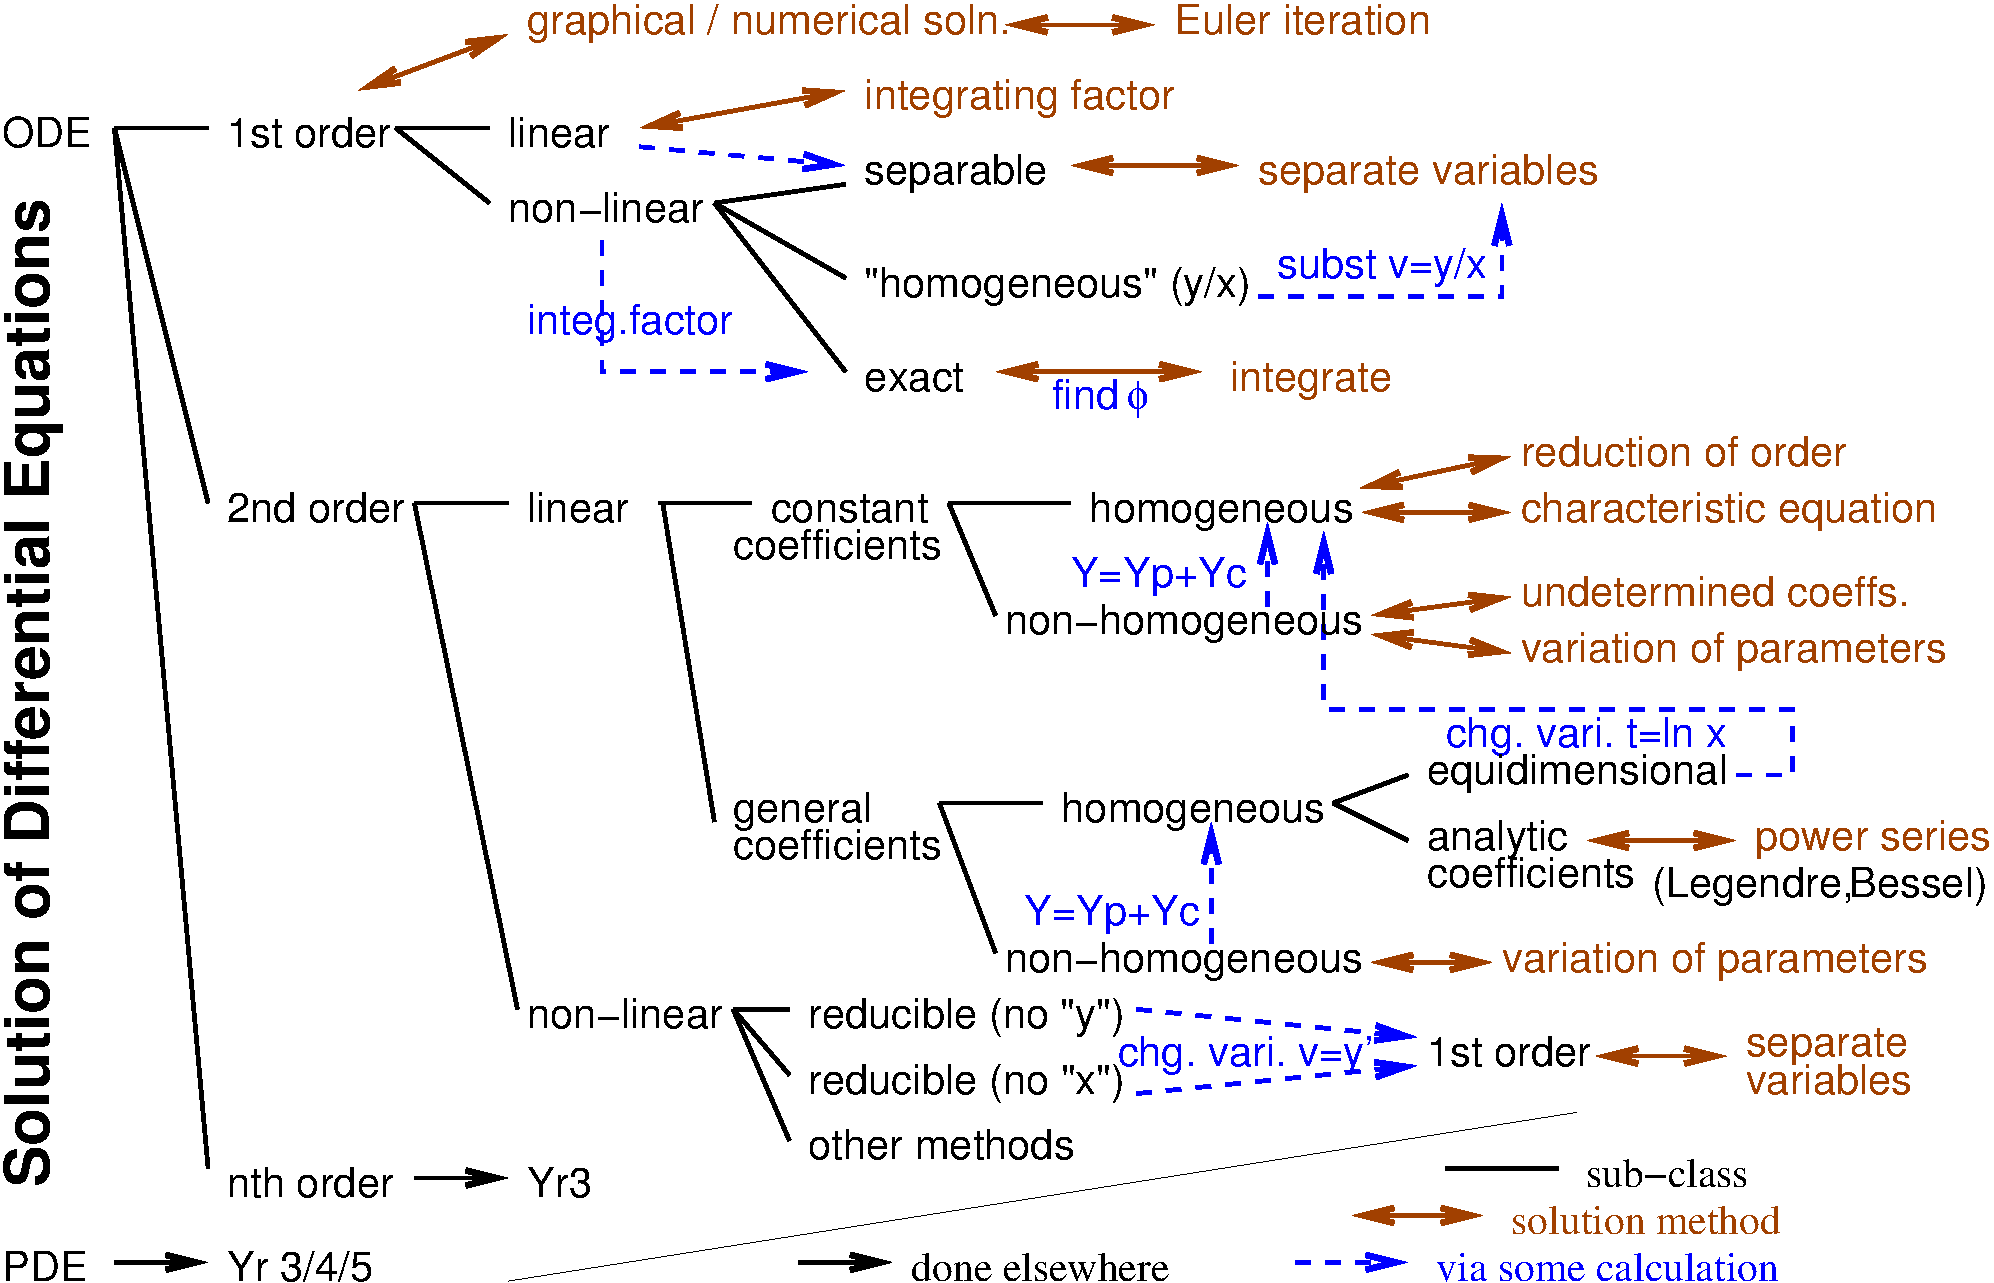
\includegraphics[width=\linewidth]{ODE_solution.pdf} % Replace with your PDF file
	\caption{An example figure.}
	\label{fig:example}
\end{wrapfigure}

\section{1}
'\\'\\'\\'\\'\\'\\'\\'\\'\\'\\'\\'\\'\\'\\'\\

\section{Classification of ODE}


\sectionspace

\section{First Order ODE}
:\\
Standard Form : $\frac{dy}{dx} + P(x)y = Q(x)$\\
1. \method{graphic method is plot the direction field}\\
2. \method{numerical method/Euler's Method}:\\
$y_1 = y_0 + f(t_0,y-0)h$, $h$ is the step\\
3. \method{If Linear?}\\
- \textbf{Separable?}\\
- \textbf{integrating factor}:\\
$e^{\int P(x) dx}[\frac{dy}{dx} + P(x)y ]= e^{\int P(x) dx}Q(x)$\\
4  \method{non-Linear?}\\
- \textbf{Separable?}\\
- \textbf{homogeneous}\\
Can be express as $\frac{y}{x}$ only, let $v(x) = \frac{y}{x}$,\\ 
$y = v(x)x$
sub in $ y'$ and separate the variable\\
- \textbf{Exact equation} : $M(x,y) + N(x, y)\frac{dy}{dx} = 0$  \\
ODE  is exact on R if and only if $ \frac{\partial{M}}{\partial{y}} =  \frac{\partial{N}}{\partial{x}}$\\
there exist $\psi(x, y )$ such that $\frac{\partial{\psi}}{\partial{x}} =  M$ and $\frac{\partial{\psi}}{\partial{y}} = N$\\
Solve it  and get $\psi(x, y) = C$ as solution\\
From $M = \psi(x ,y)_x$, we get $\psi(x,y) = some(x, y) + h(y)$ and compare it with $\psi(x,y)_y =  some(x,y)_y + h(y)'$ with $N$\\
- \textbf{Integrating factor to make equation exact}:\\
For $M(x,y) + N(x, y)\frac{dy}{dx} = 0$ if it is not exact:\\
Find some $\mu(x)$ that $\mu M(x,y) + \mu N(x, y)\frac{dy}{dx} = 0$ is exact:\\
$\frac{d \mu}{dx} = \frac{M_y - N_x}{N \cdot \mu}$\\
solve the separable ODE and solve the original equation with Exact method.

\sectionspace

\subsection{Uniqueness}
 
 IVP(initial value problem)\\

1. \method{non Linear}\\
- the range should include the initial value\\
- not a general solution

\sectionspace

\section{Second Order ODE}
:\\
CC := Constant Coefficient\\
NCC := Non Constant Coefficient\\
Standard Form: \\ $
P(t) \frac{d^2y}{dt^2} + Q(t) \frac{dy}{dt} + R(t)y = G(t);$\\ 
$\text{provided that } P(t) \neq 0 \text{, it may be expressed as}$\\
$\frac{d^2y}{dt^2} + p(t) \frac{dy}{dt} + q(t)y = g(t).$

\sectionspace

\subsection{Linear}
:\\
1. Suppose that $ y_1, y_2 $ are 2 linearly independent 
solutions to the homogeneous ODE $y''(t)+ P(t)y'(t)+ Q(t)y(t) = 0$, where $p, q$ are continuous,
Then every solutions to the ODE has the form( general solution)
$y = C_1y_1(t) + C_2y_2(t)$, where $C_1, C_2$ are constants.\\
2. $y_1(t), y_2(t)$ are linearly independent iff\\
$W(y_1(t), y_2(t)) = y_1 \cdot y_2' - y_1' \cdot y_2$\\
3. $y_1, y_2$: fundamental set of solutions\\

- \method{Caracteristic Equation (\properties{CC, Homogeneous})}:\\
$ay''(t)+ by'(t)+ cy(t) = 0$, $ar^2 + br +  c  = 0$\\
if $\Delta > 0$: $y(t) =  C_1 exp(r_1t)+ C_2 exp(r_2t)$\\
if $\Delta = 0$:
- \method{Method of Reduction of Order}:\\
	When r has two same solutions, let $y_2(t) = v(t) \cdot y_1(t)$, find $y_2'$ and $y_2''$ sub in\\
	$y(t) =  C_1 exp(r_1t)+ C_2 t \cdot exp(r_1t)$\\
if $\Delta < 0$: $r = \alpha \pm \mathrm{i} \beta$:\\
$y(t) = e^{\alpha t} (C_m \cos(\beta t) + C_N \sin(\beta t))$\\

- \method{Complementary Equation (\properties{CC, Non homogeneous})}\\
$ay''(t)+ by'(t)+ cy(t) = g(t)$\\
– Find the general soln $y_c$ of the corresponding homogeneous ODE\\
– find any particular soln $y_p$ to the non homogeneous ODE;\\
– then add $y_c$ and $y_p$ together.\\

- \textbf{How to find $y_p$ particular solution}\\
- \method{Method of Undetermined  Coefficients(\properties{CC, Special Cases})}:\\
Suppose $r_1, and r_2$  are two solution to the characteristic equation\\
- \textbf{Case1: $g(t) = Me^{kt}$}\\
if $k \neq r_1 and k \neq r_2 $, $y_p = Ce^{kt}$\\
if $k$ equals one of them, $y_p = Cte^{kt}$\\
if $k = r_1 = r_2$, $y_p = Ct^2e^{kt}$\\
- \textbf{Case2: $M \cos{kt}+N\sin{kt}$ }: \\
compare $k$ and $\beta$: $y_p(t) = C \cos{kt} + D \sin{kt}$ or \\
$y_p(t) = t(C \cos{kt} + D \sin{kt})$\\
- \textbf{Case3: $g(t) = a_n t^n + ... a_0$}
if 0 is not, one, two of solution of characteristic equation:\\
$y_p(t) = b_n t^n  + ... + a_0$ or\\
$y_p(t) = t(b_n t^n  + ... + a_0)$ or\\
$y_p(t) = t^2(b_n t^n  + ... + a_0)$\\
- \textbf{Combination of Case 1,2,3}:\\
P, A, B are polynomial with different coefficients\\
$\text{if } g(t) = P_n(t) \text{, try } y_p(t) = t^s A_n(t)$\\
$\text{if } g(t) = P_n(t)e^{mt} \text{, try } y_p(t) = t^s A_n(t)e^{mt}$\\
$\text{if } g(t) = P_n(t)e^{mt} \cos kt \text{, try } y_p(t) = t^s e^{mt} \big[A_n(t) \cos kt + B_n(t) \sin kt\big]$\\
$\text{if } g(t) = P_n(t)e^{mt} \sin kt \text{, try } y_p(t) = t^s e^{mt} \big[A_n(t) \cos kt + B_n(t) \sin kt\big]$\\
- \method{Method of variation of parameters(\properties{CC, General Method})}\\
$g(t)$: see the standard form\\
$y_p(t) = y_1(t)u_1(t) + y_2(t)u_2(t)$\\
$y_p(t) = -y_1(t) \int \frac{y_2(t) g(t)}{a W(y_1, y_2)} \, dt + y_2(t) \int \frac{y_1(t) g(t)}{a W(y_1, y_2)} \, dt$\\

- \method{Reducible ODEs(\properties{NCC, non-linear})}\\
Normally we have $F(y'', y', y, x)$\\
F in the  form of $F (y'', y', x)$ we let $v(x) = \frac{dy}{dx}$, $\frac{dv}{dx} = y''$\\
F in the  form of $F(y'', y', y)$ we let $v(y)  = \frac{dy}{dx}$, $\frac{dv}{dy} = y''$\\

- \method{Euler's method(\properties{NCC})}\\
In the form of $ax^2y''+bxy' +cy = 0$, let $t= lnx$ and change variable

\sectionspace

\section{Series Solution}
:\\
$n=k$ then for all $n$ at left$n = 0$ at right $n = n+k$\\
$y = \sum_{n=0}^{\infty} a_{n}x^{n}$\\
$y' = \sum_{n=0}^{\infty} a_{n+1}(n+1)x^{n}$\\
$y'' = \sum_{n=0}^{\infty} a_{n+2}(n+2)(n+1)x^{n}$

\subsection{Legendre equation}
:\\
$(1- x^2)y''-2xy' + \alpha (\alpha +1) y = 0, \alpha > -1$

\subsection{Method of Frobenius: near a regular singular point}
:\\
$y = x^r \sum_{n=0}^{\infty} a_{n}x^{n}$


\sectionspace

\section{Other Tricks}
:\\
1. $\frac{d}{dx} \sinh(x) = \cosh(x), \quad
\frac{d}{dx} \cosh(x) = \sinh(x)$,$ \sinh(2x)=2\sinh(x)\cosh(x)$, \\
2. $d$ is the shortest distance between a point $q$ and a line $l$ with directional vector $v$, $p$ is also a point on the line: 
$d = \frac{\lvert (\mathbf{p} - \mathbf{q}) \times \mathbf{v} \rvert}{\lvert \mathbf{v} \rvert}.$
3. \method{Use symmetry when calculating $\partial f$}\\
4. \method{Contour curve}:
$\nabla f =  0$ would be the function of some line on the graph,\\
Check for symmetry,Check for x = 0, y = 0

\sectionspace


\section{Derivative}
:\\
1. $\frac{d}{dx} \sinh(x) = \cosh(x), \quad
\frac{d}{dx} \cosh(x) = \sinh(x)$,

\section{Integral}
:\\
1. $\int xe^x \, dx = (x - 1)e^x + C$\\
2. $\int x^2 e^x \, dx = (x^2 - 2x + 2)e^x + C$\\


\sectionspace

\section{Transformation}
:\\
$ \sinh(2x)=2\sinh(x)\cosh(x)$\\

\sectionspace

\section{Vector Calculus}
:\\
1. $\underline{r}(t) = f(t) \underline{i} \ + \ g(t) \underline{j}$\\
2. $\textbf{Arc length of Vector} = \int_{b}^{a} \sqrt[]{f'(t)^2 + g'(t)^2} dt $\\
3. The forms of Line\\
$\textbf{vector form}: \underline{r} = \underline{r_{0}} + t\underline{v}$\\
$\textbf{parametric form}: x = x_{0} + at, y = y_{0} + bt $\\
$\textbf{symmetric form}: \frac{x-x_{0}}{a} = \frac{y-y_{0}}{b} = t$\\
4. $\textbf{Unit Tangent vector}: \underline{T}(t) = \frac{\underline{r}'(t)}{|\underline{r}'(t)|}$\\
5. $\textbf{Cuvature}: \kappa = |\frac{dT}{ds}| = \frac{\lvert \underline{r}'(t) \times \underline{r}''(t) \rvert}{\lvert \underline{r}'(t) \rvert^3}$\\
6. $\textbf{Normal vector}: \underline{N}(t) = \frac{\underline{T}'(t)}{|\underline{T}'(t)|}$\\
7. $\textbf{Binormal vector}: \underline{B}(t) = \underline{T}(t) \times \underline{N}(t)$

\sectionspace


\section{Important Summations}
:\\
1. $\sum_{k=0}^{n} k^2 = \frac{n(n+1)(2n+1)}{6}$\\
2. $\sum_{k=0}^{n} k^3 = \left(\frac{n(n+1)}{2}\right)^2$\\
3. $e^\lambda = \sum_{k=0}^{n} \lambda^k/k!$\\
4. $sin(x) = \sum_{k=0}^{n} (-1)^k x^{2k+1}/(2k+1)!$\\
5. $cos(x) = \sum_{k=0}^{n} (-1)^k x^{2k}/(2k)!$

\sectionspace

\begin{figure}
	\centering
	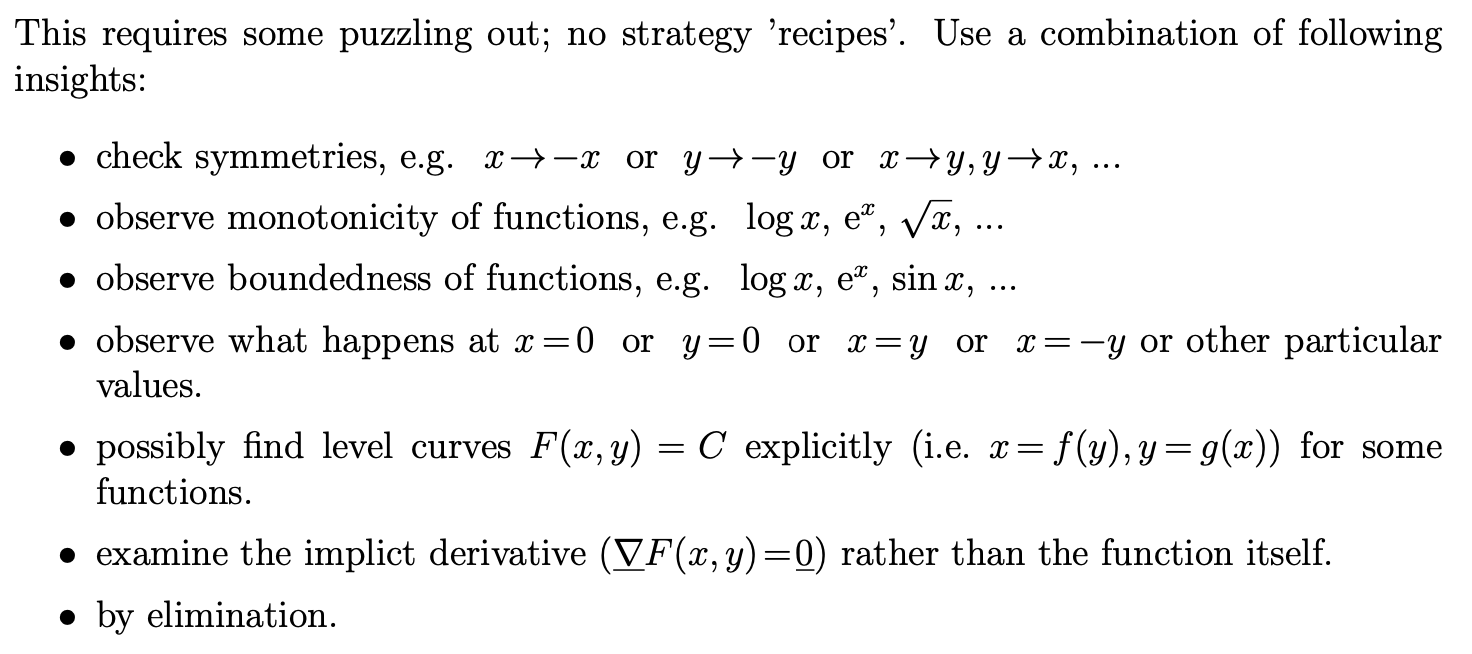
\includegraphics[width=1\linewidth]{screenshot001}
	\caption{}
	\label{fig:screenshot001}
\end{figure}

\begin{figure}
	\centering
	\includegraphics[width=1.1\linewidth]{"Pasted Graphic 1.png"}
	\caption{}
	\label{fig:pasted-graphic-1}
\end{figure}





\end{document}
